\section{Cross-correlation}\label{sec:CC}

The first attempt at locating a thigh in the 3D image used the mathematical cross-correlation operator.
A 3D ``thigh-filter'' was generated using Matlab which matched the shape and size of a typical thigh from the sample data.
This was then cross-correlated with the 3D voxel-space image to determine where in the image the thigh was most likely to be.

\bigskip
\noindent Cross-correlation is similar to convolution in that two signals are moved over each other to produce a third signal describing where they best match.
For 3-dimensional discrete input images $f$ and $g$, the cross-correlation image $(f \star g)$ is defined as:

\begin{equation}
	(f \star g)_{(\delta x,\delta y,\delta z)} = \sum_{x=1}^{s_{x}} \sum_{y=1}^{s_{y}} \sum_{z=1}^{s_{z}} f_{(x,y,z)} \cdot g_{(x+\delta x,y+\delta y, z+\delta z)}
\end{equation}

Where $s$ is the size in pixels of the image $f$.

In our case we are not interested in the translation $(\delta x,\delta y,\delta z)$ of the thigh-filter $f$ over the voxel-space image $g$, but rather its rotation.
It is assumed that the thigh has two degrees-of-rotation: $\theta$ - the rotation that makes the leg move in the walking direction, and $\alpha$ - any side-to-side movement of the leg.
We implement this by introducing a transformation matrix $\mathbf{M}(\alpha,\theta)$:

\begin{equation}
	\mathbf{M}(\alpha,\theta) =
	\left(\begin{array}{ccc}
		cos(\alpha) & 0 & sin(\alpha) \\
		0 & 1 & 0 \\
		-sin(\alpha) & 0 & cos(\alpha)
	\end{array} \right)
	\times
	\left(\begin{array}{ccc}
		1 & 0 & 0 \\
		0 & cos(\theta) & -sin(\theta) \\
		0 & sin(\theta) & cos(\theta)
	\end{array} \right)
	\label{eqn:Matrix}
\end{equation}

This allows us to parameterise the cross-correlation image $(f \star g)$ with $\alpha$ and $\theta$ instead:

\begin{equation}
	(f \star g)_{(\alpha,\theta)} = \sum_{x=1}^{s_{x}} \sum_{y=1}^{s_{y}} \sum_{z=1}^{s_{z}} f_{(x,y,z)} \cdot g_{\mathbf{M}(\alpha,\theta) \times (x,y,z)^T}
	\label{eqn:CrossCorrelation}
\end{equation}


\begin{figure}[tb]
	\centering
	\subfloat[Top near hips]{\includegraphics[width=4cm]{../interim/filter1.png}}
	\quad
	\subfloat[Bottom near knees]{\includegraphics[width=4cm]{../interim/filter2.png}}
	\caption{Cross sections through the 3D thigh-filter.  Red = 1, Blue = 0.}
	\label{ThighFilterCrossSections}
\end{figure}

\bigskip
\noindent The 3D filter is 20x20x20 pixels in volume and generated by a simple Matlab function (see \ref{ThighFilter.m}).
It is exported to a custom binary file format and later loaded by the C code where it is stretched to match the dimensions of the thigh.
Two 2D cross-sections of the filter are shown in Figure \ref{ThighFilterCrossSections}.
From these it can be seen that the filter has a cylindrical core of value 1 to match the solid central section of the thigh.
Additional rings of pixels with lower values are built up around the edge of this cylinder towards the bottom.
The idea is that the filter will then fit ``better'' when it is placed exactly in the center if the thigh,
as this is where the filter pixels with the highest values will correspond to filled voxels in the thigh.

The rings are smaller towards the top of the filter so as not to match the area of filled voxels where the thighs join the hips.

\bigskip
\noindent One of the reasons that this cross-correlation approach was attempted first is that it lends itself very nicely to implementation on a stream processor.
The same matrix multiplications and floating point operations can be performed on a large amount of data at once, with no dependencies or iterative behaviour.
Figure \ref{CrossCorrelation} shows how this is implemented using the OpenGL graphics pipeline.
The fragment shader used is listed in \ref{correlation.cg}.

\begin{figure}[tb]
	\vspace{-10pt}
	\centering
	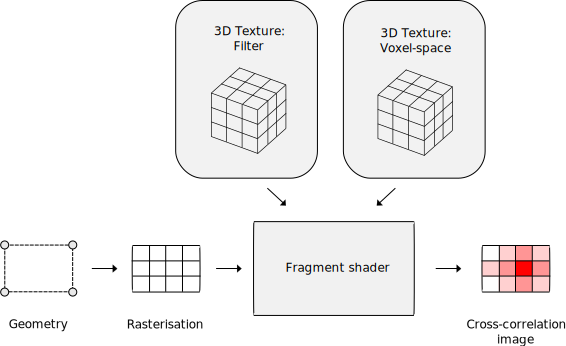
\includegraphics[height=6cm]{../interim/correlation.png}
	\caption{How the OpenGL graphics pipeline can be used to accelerate cross-correlation.
		A quad is drawn and rasterised to match the desired size of the cross-correlation image.
		A fragment program is run on each of the generated fragments to evaluate Equation \ref{eqn:CrossCorrelation}.}
	\label{CrossCorrelation}
\end{figure}

The implementation creates an additional matrix $\mathbf{M}_2$ that is used to convert between the coordinate spaces of OpenGL textures to those of our filters and voxel-space.
It also contains a translate and a scale operation to align the filter with the hips, and scale it to the right size.
The values used in these transformations are obtained from Section \ref{LocatingCenter}.
This $\mathbf{M}_2$ is applied to our original $\mathbf{M}$ from Equation \ref{eqn:Matrix} like so:

\begin{equation}
	\mathbf{M}' = \mathbf{M} \times \mathbf{M}_2
\end{equation}

\bigskip
\noindent The results from this method reveal that perhaps this kind of simple correlation is not suitable for detecting parts of the body in our sample data.
Figure \ref{ParameterSpace} shows the cross-correlation image for a thigh that is oriented straight, in standing position.
It can be seen that $\theta$ is generally correct - horizontally, the concentration of intensity is in the middle of the image, meaning $\theta \simeq 0$.
However vertically there is a far greater concentration of colour towards the bottom of the image where $\alpha$ is positive.
This is because here the thigh-filter has been rotated inwards towards the centre of the figure, and is matching parts of both left and right legs.

\begin{figure}[tb]
	\vspace{-10pt}
	\centering
	\includegraphics[height=4cm]{../interim/parameterspace.png}
	\caption{An output cross-correlation image, with correlation strength rendered into the red colour channel.
		$\theta$ is mapped to the X axis, and $\alpha$ to Y.
		The centre of the image is $(\theta, \alpha) = (0,0)$.}
	\label{ParameterSpace}
\end{figure}

A workaround for this is to fix $\alpha = 0$ and only concern ourselves with $\theta$.
This is acceptable, as the movement of the leg along the walking direction is much greater and more relevant \cite{GaitBook} than its movement perpendicular to that direction.
The results from this method are promising, and demonstrate that the algorithm does work to a certain degree.
